
% THIS IS SIGPROC-SP.TEX - VERSION 3.1
% WORKS WITH V3.2SP OF ACM_PROC_ARTICLE-SP.CLS
% APRIL 2009
%
% It is an example file showing how to use the 'acm_proc_article-sp.cls' V3.2SP
% LaTeX2e document class file for Conference Proceedings submissions.
% ----------------------------------------------------------------------------------------------------------------
% This .tex file (and associated .cls V3.2SP) *DOES NOT* produce:
%       1) The Permission Statement
%       2) The Conference (location) Info information
%       3) The Copyright Line with ACM data
%       4) Page numbering
% ---------------------------------------------------------------------------------------------------------------
% It is an example which *does* use the .bib file (from which the .bbl file
% is produced).
% REMEMBER HOWEVER: After having produced the .bbl file,
% and prior to final submission,
% you need to 'insert'  your .bbl file into your source .tex file so as to provide
% ONE 'self-contained' source file.
%
% Questions regarding SIGS should be sent to
% Adrienne Griscti ---> griscti@acm.org
%
% Questions/suggestions regarding the guidelines, .tex and .cls files, etc. to
% Gerald Murray ---> murray@hq.acm.org
%
% For tracking purposes - this is V3.1SP - APRIL 2009

\documentclass{acm_proc_article-sp}

\usepackage{multirow}
\usepackage{subfigure}
\usepackage{graphicx}
\usepackage{graphics}
\usepackage{rotating}
\usepackage{verbatim}
\usepackage{float}
\usepackage{url}
\usepackage{tabularx}
\usepackage{amsmath}
\usepackage{listings}
\usepackage{color}
\definecolor{javared}{rgb}{0.6,0,0} % for strings
\definecolor{javagreen}{rgb}{0.25,0.5,0.35} % comments
\definecolor{javapurple}{rgb}{0.5,0,0.35} % keywords
\definecolor{javadocblue}{rgb}{0.25,0.35,0.75} % javadoc
 
\lstset{language=Java,
basicstyle=\ttfamily,
keywordstyle=\color{javapurple}\bfseries,
stringstyle=\color{javared},
commentstyle=\color{javagreen},
morecomment=[s][\color{javadocblue}]{/**}{*/},
%numbers=left,
numberstyle=\tiny\color{black},
stepnumber=2,
numbersep=10pt,
tabsize=4,
showspaces=false,
showstringspaces=false}



\restylefloat{table}

\hyphenation{op-tical net-works semi-conduc-tor}



\begin{document}



\title{Automated Discovery of Failure Domain+ and Daikon to Analyse Boundaries}


\numberofauthors{2} %  in this sample file, there are a *total*
% of EIGHT authors. SIX appear on the 'first-page' (matting
% reasons) and the remaining two appear in the \additionalauthors section.
%
\author{
% You can go ahead and credit any number of authors here,
% e.g. one 'row of three' or two rows (consisting of one row of three
% and a second row of one, two or three).
%
% The command \alignauthor (no curly braces needed) should
% precede each author name, affiliation/snail-mail address and
% e-mail address. Additionally, tag each line of
% affiliation/address with \affaddr, and tag the
% e-mail address with \email.
%
% 1st. author
\alignauthor
Mian Asbat Ahmad\\
       \affaddr{Department of Computer Science}\\
       \affaddr{The University of York}\\
       \affaddr{York, United Kingdom}\\
       \email{mian.ahmad@york.ac.uk}
% Please Dr. Manuel, add your abb details. I am not able to create table here because of the format. Thanks.
\alignauthor
Manuel Oriol \\
       \affaddr{Department of Computer Science}\\
       \affaddr{The University of York}\\
       \affaddr{York, United Kingdom}\\
       \email{manuel.oriol@york.ac.uk}
}



\maketitle
\begin{abstract}
This paper verify the accuracy of invariants generated automatically by Daikon and suggests how to improve their quality. To achieve this, it uses a newly developed technique called Automated Discovery of Failure Domain+ (ADFD+). It is a testing framework that after identifying a failure search its surrounding values to the specified range. The result obtained is presented graphically indicating pass and fail points.

Several error seeded two dimensional programs were tested in the experiments with point block and strip fault domain were evaluated first with ADFD+ and than with Daikon. On comparison of results from both the methods it is found that where Daikon generates the correct invariants, it was not good enough to identify the fault boundaries.

It is concluded that it will be highly effective if the fault boundary found by ADFD+ is passed to the Daikon in the first stage then the invariants generated by Daikon will correctly point to the fault boundary.

\end{abstract}

%A category including the fourth, optional field follows...
%\category{D.2.5}{Software Engineering}{Metrics}[complexity measures, performance measures]

%\terms{Comparison, Verification, }

\keywords{software testing, automated random testing} % NOT required for Proceedings





%%%%%%%%%%%%%%%%%    INTRODUCTION   %%%%%%%%%%%%%%%%%%%%

\section{Introduction}\label{sec:intro}
Testing is the most widely used and essential method of software testing. Ample efforts have been made to improve its effectiveness and efficiency. Testing is effective if it finds maximum number of faults in minimum number of test cases. Testing efficiency is the process to execute maximum number of test cases in minimum possible time. It is concluded that automation is the key to achieve both effectiveness and efficiency of software testing. Automation of a single part like data generation, execution, oracle or the whole system is highly beneficial in most of the cases. Some of the common automated testing tools include YETI~\cite{Oriol2011yeti}, Randoop~\cite{pacheco2007randoop}, Eclat~\cite{pacheco2005eclat}, QuickCheck~\cite{claessen2011quickcheck} and Jaretege~\cite{oriat2005jartege}. 

Daikon~\cite{ernst2007daikon} is one of the several tools, which uses machine learning technique to automatically generate likely invariants of the program written in C, C++, Java and Pearl. Daikon takes as input the program and few test cases written manually or generated by an automated tool. It executes the test cases on the program under test and observes the values that the program computes. At the end of the test session it reports the properties that were true over the observed executions. Daikon can process the generated invariants to mitigate non interesting and redundant invariants. Daikon can also inserts the generated invariants in to the source code as assertions. Daikon's output can be useful in understanding program, generating invariants, predicting incompatibilities in component integration, automating theorem proving, repairing inconsistent data structures and checking the validity of data streams.

While the idea behind Daikon is attractive, it is interesting to see how much the auto generated invariants represent the fault domain residing in the program. To assess this, we set up performed several experiments and analysed the results derived from the error-seeded programs tested with Daikon and ADFD+. ADFD+ is a framework named Automated Discovery of Failure Domain+. It is based on our previous strategy Automated Discovery of Failure Domain (ADFD), which tries to find a fault, search the surrounding for more faults and graphically plot the fault domain if any~\cite{ahmad2013adfd}.  

The main contribution of the article are:
\begin{itemize}
\item \textbf{ADFD+:} It brings some changes to the previously proposed ADFD strategy. The new strategy improves the search algorithm of ADFD and make the report more intuitive.
\item \textbf{Implementation of ADFD+:} The new ADFD+ strategy is implemented and integrated in the YETI tool.
\item \textbf{Evaluation:} It evaluates the report generated by Daikon and ADFD+ about the boundaries known fault domains in the error-seeded programs. It is found that where Daikon was able to find the fault, it was not able to identify its domain boundary as accurately as ADFD+.
\item \textbf{Future work:} It gives ideas of further application of ADFD+, such as finding and plotting faults in multi-dimensional programs using multi-dimensional graphs. 
% A case study suggesting that boundaries are properly recognized by Daikon and ADFD+ or Daikon lake .... etc.
\end{itemize}
%The rest of this paper is organised as follows: \\ Section~\ref{sec:adfd} describes the ADFD+ strategy. Section~\ref{sec:imp} presents implementation of the ADFD+ strategy. Section~\ref{sec:eval} explains the experimental setup. Section~\ref{sec:res} shows results of the experiments. Section~\ref{sec:discussion} discusses the results. Section~\ref{sec:rw} presents related work and Section~\ref{sec:conc}, concludes the study.


%In the later part we plot the domain on the basis of invariants generated by Daikon and compare both the domains.

%%%%%%%%%%%%%%%%%    Background   %%%%%%%%%%%%%%%%%%%

\section{Failure Patterns}
A number of empirical evidence confirms that fault revealing test cases tend to cluster in contiguous regions across the input domain~\cite{white1980domain, finelli1991nasa, schneckenburger2007towards}. According to Chan et al.~\cite{chan1996proportional} the clusters are arranged in the form of point, block and strip failure pattern. In the point pattern the failure revealing inputs are stand alone which are spread through out the input domain. In block pattern the failure revealing inputs are clustered in a one or more contiguous area. Finally, in strip pattern the failure revealing inputs are clustered in one long elongated area.  Figure~\ref{fig:failurePatterns} shows the failure patterns in two-dimensional input domain. 

\begin{figure}[ht]                                    
\centering
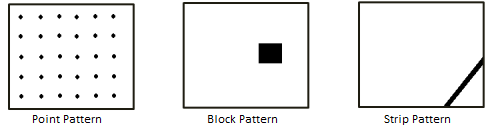
\includegraphics[width= 8cm,height=2.5cm]{ART_Patterns.png}
\caption{Failure patterns across input domain~\cite{chan1996proportional}}
\label{fig:failurePatterns}
\end{figure}

%In Section~\ref{sec:adfd+} we describe the ADFD+ framework that can find the failure, its domain and plot the domain up to the specified range in a graphical form. Experiments confirms the successful working of ADFD+.


 

%%%%%%%%%%%%%%%%%    ADFD+   %%%%%%%%%%%%%%%%%%%

\section{Automated Discovery of Failure Domain+}\label{sec:adfd+}
ADFD+ is an improved and extended form of our previously developed Automated Discovery of Failure Domain~\cite{ahmad2013adfd}. The ADFD+ is an automated framework that finds the failures, their domains in a specified range and present them on a graphical chart. Following  are the main differneces between ADFD and ADFD+.

\begin{itemize}
\item ADFD+ generate a single Java file dynamically at run time to plot the failure domains instead of one Java file per failure as in ADFD. This saves a lot of execution time and makes the process much quicker.

\item ADFD+ uses (x, y) vector series to represent failure pattern as opposed to the (x, y) line series in ADFD. The vector series allows more flexibility and clarity to represent a failure and its domain domain.   

\item ADFD+ takes a single value as range which specify a round region around the failure whereas takes two values for lower and upper bound representing x and y axis respectively.

\item In ADFD+, the algorithm of dynamically generated Java file, which is created after an error is discovered, is made more simplified and efficient.

\item In ADFD+, the failure domain is focused in the graph which gives a clear view of pass and fail points. The points are also labelled for simplification as shown in the Figure~\ref{fig:Workflow}. 

%The difference in representation of fault by ADFD and ADFD+ can be seen in figure .... Figure x is generated by ADFD with lower bound as ... and upper bound as ... While Figure Y is generated by ADFD+ with range ... for the same program given in appendix a. 
\end{itemize}


%%%%%%%%%%%%%%%%%%%%

\subsection{Workflow of ADFD+}
ADFD+ is an automatic process and all the user has to do is to specify the program to test and click the $Draw Fault Domain$ button. The default value for range is set to 5 which means that ADFD+ will search 25 values around the failure. On clicking the button YETI is executed with ADFD+ strategy to search for a failure. On finding a failure the ADFD+ strategy create a java file which contain calls to the program on the failing value and related values up to the specified range. The Java file is compiled and executed. The result is analysed to check for pass and failed values. Pass values are stored in pass file and fail values are stored in fail file. At the end of the values range, the values are plotted on the graph with pass values as green and fail values as red as shown in the Figure~\ref{fig:Workflow}.


%Instead of front end give workflow. It will make more sense. Change the code of the program

\begin{figure}[ht]
\centering
\includegraphics[width= 8.5cm,height=6.5cm]{adfdPlusWorkflow.png}
\caption{Workflow of ADFD+}
\label{fig:Workflow}
\end{figure}


%%%%%%%%%%%%%%%%%%%%
%ADFD+ is an extension of ADFD's algorithm with more accuracy to find and clarity to plot the failure domain on a graphical chart. Deriving failure domains using ADFD+ is a one click process and all the tester needs to input is the class to test and the range-value for which to search around the found failure. 
%%%%%%%%%%%%%%%%%%%%

\subsection{Implementation of ADFD+}
The ADFD+ strategy is implemented in a tool called York 
Extensible Testing Infrastructure (YETI). YETI is available 
in open-source at \url{http://code.google.com/p/yeti-test/}. In this section a brief overview of YETI is given with the focus on the parts relevant to the implementation of ADFD+ strategy. For verification of ADFD+ strategy in YETI, a program is used 
as an example to illustrate the working of ADFD+ strategy. Please refer to \cite{Oriol2011yeti, oriol2012random, oriol2010testing, oriol2010yeti} for more details on YETI. 

YETI is a testing tool developed in Java that test programs using random strategies in an automated fashion. YETI meta-model is language-agnostic which enables it to test 
programs written in functional, procedural and object-oriented languages. 

YETI consists of three main parts including core infrastructure for extendibility through specialization, strategies section for adjustment of multiple strategies and 
languages section for supporting multiple languages. Both the languages and strategies sections have a pluggable architecture to easily incorporate new strategies and 
languages making YETI a favorable choice to implement ADFD+ strategy. YETI is also capable of generating test cases to reproduce the faults found during the test session. 
The strategies section in YETI contains all the strategies including random, random+ and DSSR to be selected for testing according to the specific needs. The default test 
strategy for testing is random. On top of the hierarchy in strategies, is an abstract class YetiStrategy, which is extended by YetiRandomPlusStrategy and is further, extended to get 
ADFD+ strategy.


\subsection{ADFD+ by an example}
In this section we describe the working of ADFD+ with a motivating example. Suppose we have the following class name $Error$ under test. According to the code, the value of variable $x$ between 5 to 8 and the value of variable $y$ between 2 to 4 triggers a failure.   

\begin{lstlisting}

public class Error {

  public static void Error (int x, int y){

    int z;

    if (((x>=5)&&(x<=8))&&((y>=2)&&(y<=4)))
		 {
			 z = 50/0;
		 }
   } 
}
\end{lstlisting}

On execution, the ADFD+ strategy tests the class with the help of YETI and finds a failure at x = 6 and y = 3. Once a failure is discovered ADFD+ uses the surrounding values around the failure to find a failure domain. The range of surrounding values is limited to the value set by the user in the $Domain Range$ variable. When the value of $Domain Range$ is 5, ADFD+ evaluates total of 83 values of $x$ and $y$ around the found failure. All evaluated (x, y) values are plotted on a two dimensional graph with red dot indicating a failing value and green dot indicating the passing value as shown in the Figure~\ref{fig:adfdPlusExample}. 

\begin{figure*}[ht]
\centering
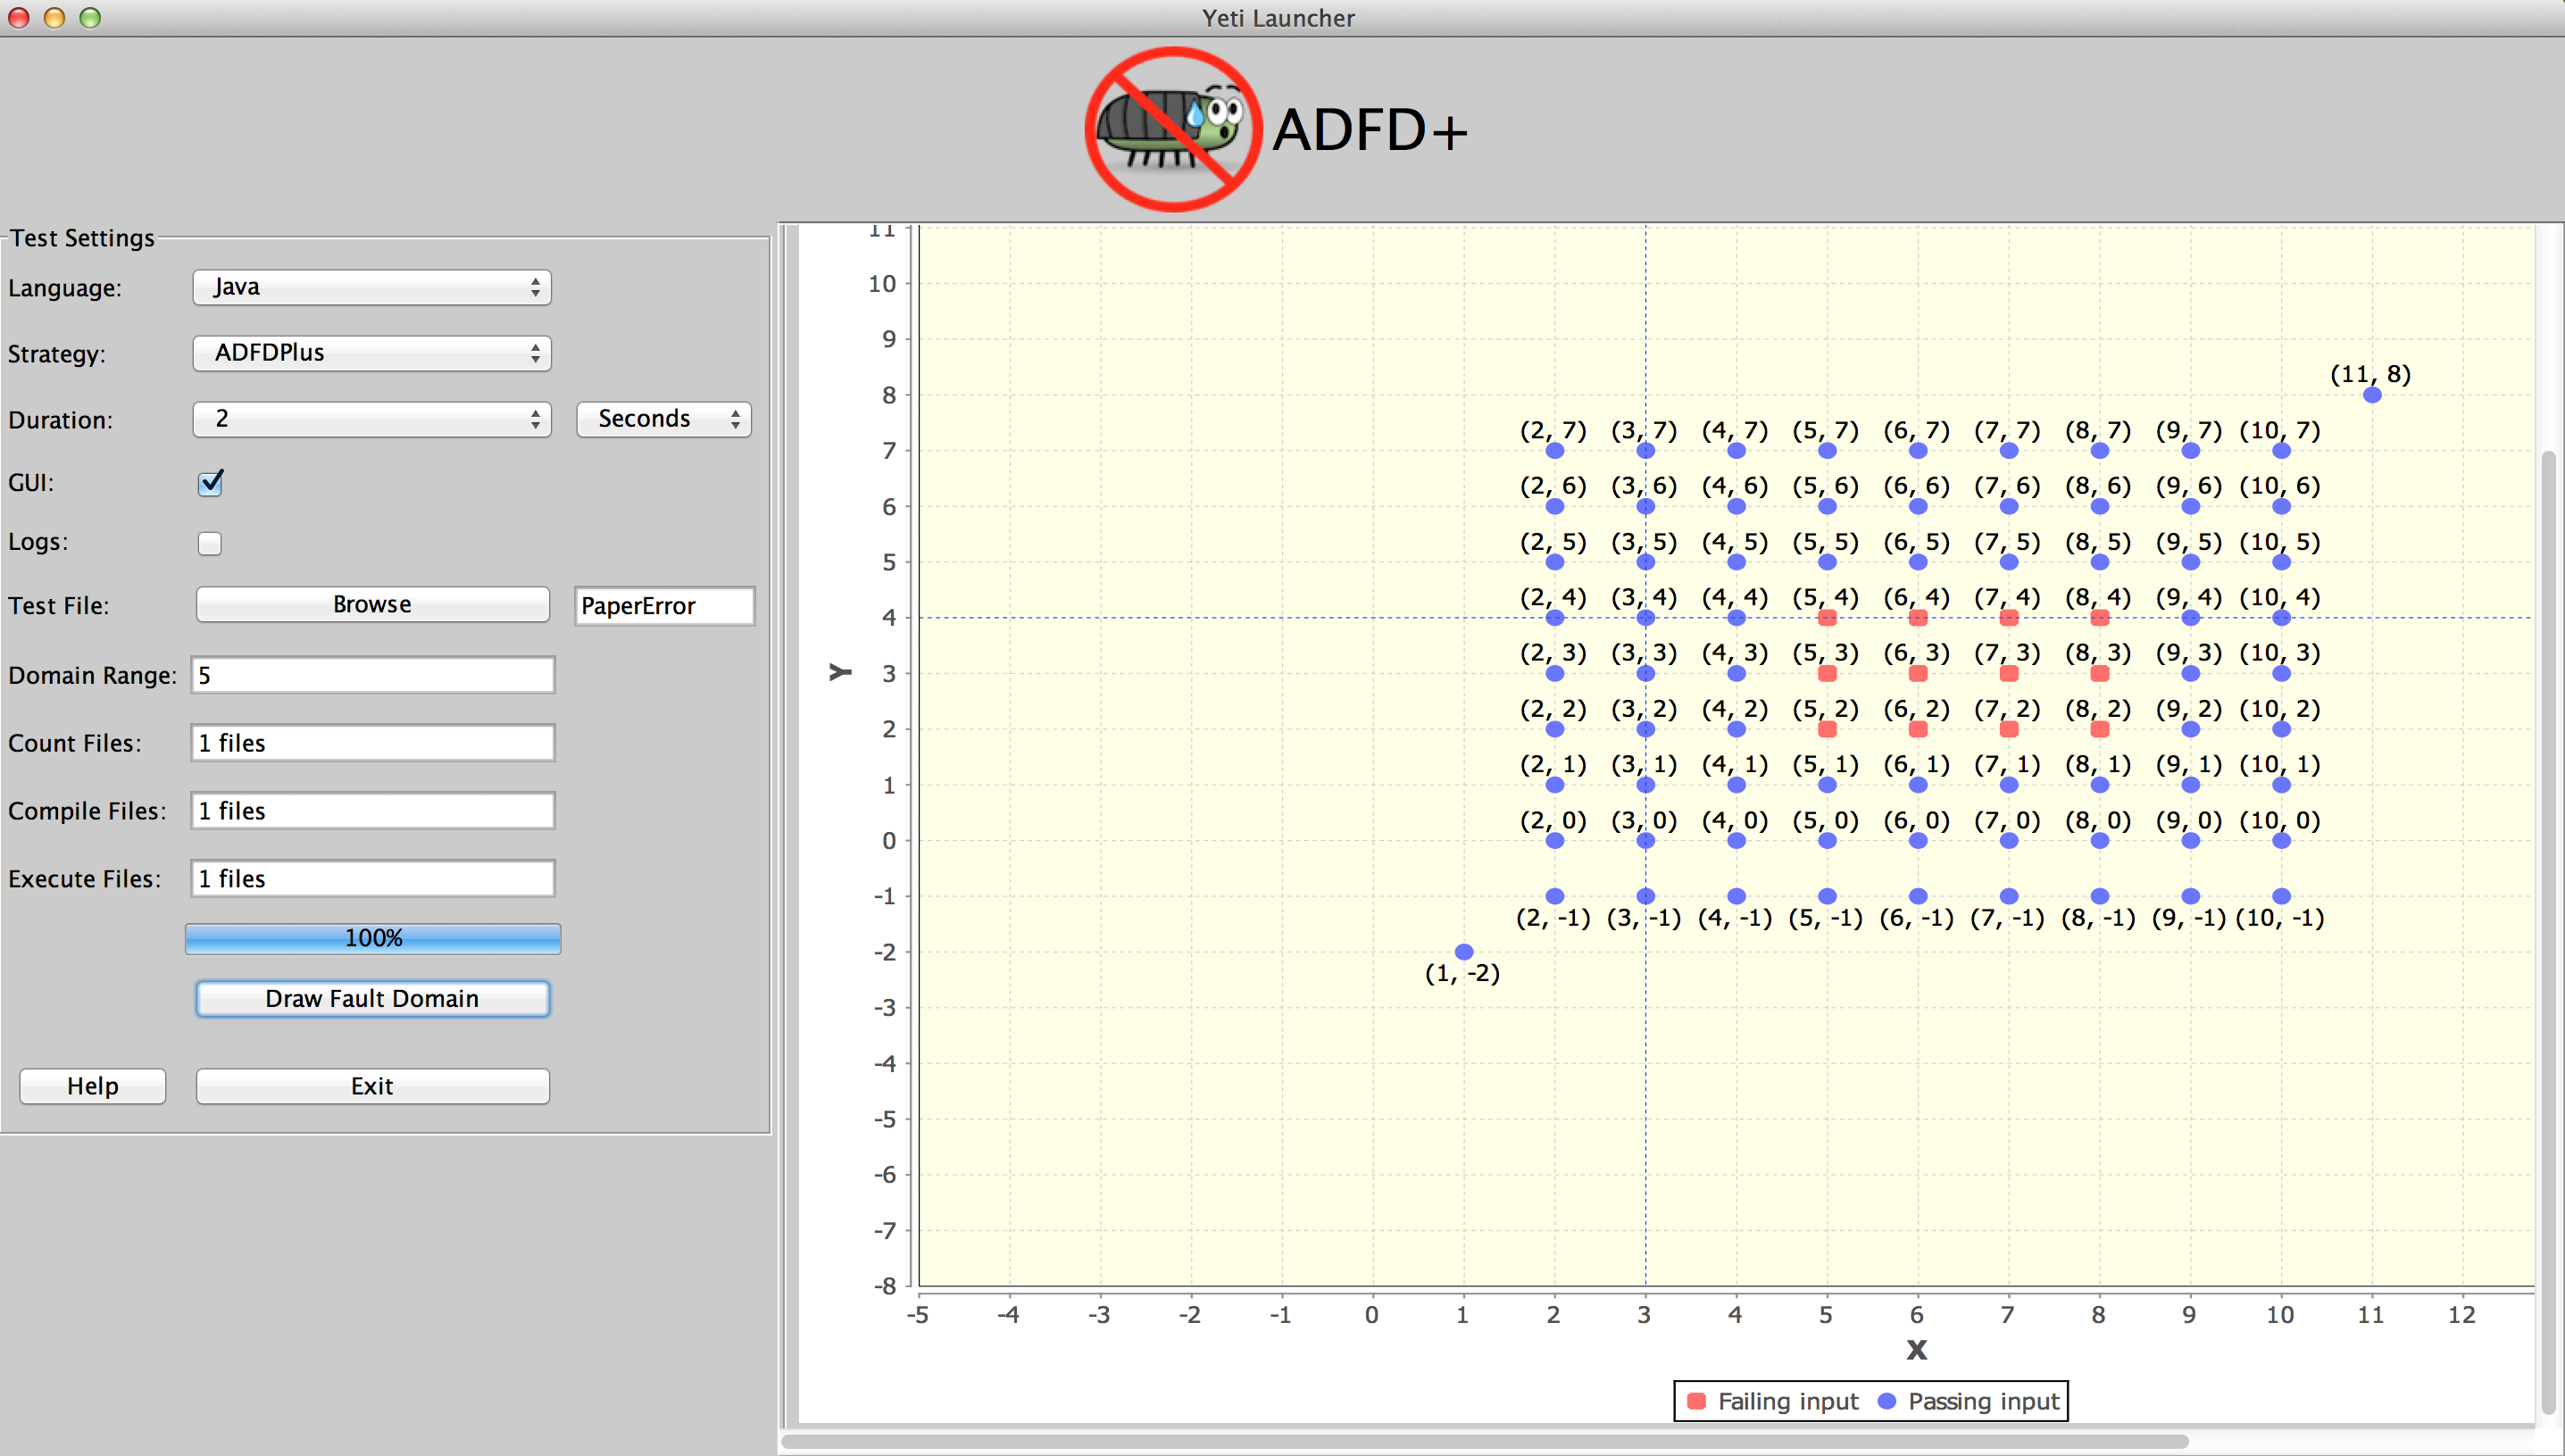
\includegraphics[width=17.5cm,height=11cm]{exampleError.png}
\caption{The output of ADFD+ for the above code.}
\label{fig:adfdPlusExample}
\end{figure*}

\section{Experimental Setup}

\section{results}
\section{Discussion}
\section{Threats to validity}
\section{Conclusion}
\section{Future Work}







%%%%%%%%%%%%%%%%%    EVALUATION   %%%%%%%%%%%%%%%%%%%%


\section{Evaluation}\label{sec:eval}

The DSSR strategy is experimentally evaluated by comparing its performance with that of random and random+ strategy ~\cite{Leitner2007}. General factors such as system software and hardware, YETI specific factors like percentage of null values, percentage of newly created objects and interesting value injection probability have been kept constant in the experiments.

\subsection{Research questions}
For evaluating the DSSR strategy, the following research questions have been addressed in this study:
\begin{enumerate}
\item Is there an absolute best among R, R+ and DSSR strategies?
\item Are there classes for which any of the three strategies provide better results?
\item Can we pick the best default strategy between R, R+ and DSSR?
\end{enumerate}



\subsection{Experiments}

To evaluate the performance of DSSR we performed extensive testing of programs from the Qualitas Corpus~\cite{Tempero2010a}. The Qualitas Corpus is a curated collection of open source java projects built with the aim of helping empirical research on  software engineering. These projects have been collected in an organised form containing the source and binary forms. Version 20101126, which contains 106 open source java projects is used in the current evaluation. In our experiments we selected 60 random classes from 32 random projects. All the selected classes produced at least one fault and did not time out with maximum testing session of 10 minutes. Every class is tested thirty times by each strategy (R, R+, DSSR). Name, version and size of the projects to which the classes belong are given in table~\ref{table:projects} while test details of the classes is presented in table~\ref{table:Results}. Line of Code (LOC) tested per class and its total is shown in column 3 of table~\ref{table:Results}. 

Every class is evaluated through $10^5$ calls in each test session.\footnote{The total number of tests is thus $60\times 30\times 3 \times 10^5 = 540\times 10^6~tests$.} 
Because of the absence of the contracts and assertions in the code under test, Similar approach as used in previous studies ~\cite{Oriol2012} is followed using undeclared exceptions to compute unique failures.


\begin{table}[h]
\caption{Name and versions of 32 Projects randomly selected from the Qualitas Corpus for the experiments}
\centering
\begin{tabular}{|r|l|r|r|}
\hline
S. No& 	Project Name	& 	Version		&	Size (MB)\\
\hline
1	&	apache-ant	&	1.8.1			&	59\\
2	&	antlr			&	3.2			&	13\\
3	&	aoi			&	2.8.1			&	35\\
4	&	argouml		&	0.30.2		&	112\\
5	&	artofillusion	&	281			&	5.4\\
6	&	aspectj		&	1.6.9			&	109.6\\
7	&	axion		&	1.0-M2		&	13.3\\
8	&	azureus		&	1			&	99.3\\
9	&	castor		&	1.3.1			&	63.2\\
10	&	cayenne		&	3.0.1			&	4.1\\
11	&	cobertura		&	1.9.4.1		&	26.5\\
12	&	colt			&	1.2.0			&	40\\
13	&	emma		&	2.0.5312		&	7.4\\
14	&	freecs		&	1.3.20100406	&	11.4\\
15	&	hibernate		&	3.6.0			&	733\\
16	&	hsqldb		&	2.0.0			&	53.9\\
17	&	itext			&	5.0.3			&	16.2\\
18	&	jasml		&	0.10			&	7.5 \\
19	&	jmoney		&	0.4.4			&	5.3\\
20	&	jruby			&	1.5.2			&	140.7\\
21	&	jsXe			&	04\_beta		&	19.9\\
22	&	quartz		&	1.8.3			&	20.4\\
23	&	sandmark		&	3.4			&	18.8\\
24	&	squirrel-sql	&	3.1.2			&	61.5\\
25	&	tapestry		&	5.1.0.5		&	69.2\\
26	&	tomcat		&	7.0.2			&	24.1\\
27	&	trove			&	2.1.0			&	18.2\\
28	&	velocity		&	1.6.4			&	27.1\\
29	&	weka		&	3.7.2			&	107\\
30	&	xalan		&	2.7.1			&	85.4\\
31	&	xerces		&	2.10.0		&	43.4\\
32	&	xmojo		&	5.0.0			&	15\\
\hline
\end{tabular}
\bigskip
\label{table:projects}
\end{table}



All tests are performed with a 64-bit Mac OS X Lion Version 10.7.4 running on 2 x 2.66 GHz 6-Core Intel Xeon processor with 6 GB (1333 MHz DDR3) of RAM. YETI runs on top of the Java\texttrademark  SE Runtime Environment [version 1.6.0\_35]. The machine took approximately 100 hours to process the experiments.





\begin{table*}[htp]
\small
\caption{T-test results of the classes showing different results}
\centering
\begin{tabular}{rlrrrl}
 \multirow{2}{*} {S. No}	& \multirow{2}{*}{Class Name}	&  \multicolumn{3}{c}{T-test Results} & \multirow{2}{*}{Interpretation} \\

								& & 	DSSR, R	& DSSR, R+	&  R, R+ 	& 		\\

1		&	AjTypeImpl		&	1 				& 1 			& 1			& 		\\	
2		&	Apriori			&	\textbf{0.03}	 	& 0.49		& 0.16		&		\\	
3		&	CheckAssociator	&	\textbf{0.04}	 	& \textbf{0.05}	& 0.44		& DSSR better		\\	
4		&	Debug			&	\textbf{0.03}	 	& 0.14		& 0.56		&		\\	
5		&	DirectoryScanner	&	\textbf{0.04}	 	& \textbf{0.01}	& 0.43		& DSSR better		\\
6		&	DomParser		&	\textbf{0.05}	 	& 0.23		& 0.13		&				\\
7		&	EntityDecoder		&	\textbf{0.04}	 	& 0.28		& 0.3			&		\\			
8		&	Font				&	0.18	 			& 0.18		& 1			&		\\
9		&	Group			&	0.33	 			& \textbf{0.03}	& \textbf{0.04}	& DSSR = R > R+	\\
10		&	Image			&	\textbf{0.03}		& \textbf{0.01}	& 0.61		& DSSR better \\		
11		&	InstrumentTask		&	0.16				& 0.33		& 0.57		& \\
12		&	JavaWrapper		&	\textbf{0.001}		& 0.57		& 0.004		& DSSR = R+ > R \\
13		& 	JmxUtilities		&	0.13				& 0.71		& 0.08		&	\\
14		&	List				& 	\textbf{0.01}		&0.25		&\textbf{0}		& DSSR = R+ > R \\
15		&	NodeSequence	&	0.97				&\textbf{0.04}	&\textbf{0.06}	& DSSR = R > R+ \\
16		&	NodeSet			&	\textbf{0.03}		&0.42		&0.26		& 	\\
17		&	Project			&	\textbf{0.001}		&0.57		&\textbf{0.004}	& DSSR better \\		
18		&	Repository		&	\textbf{0}			&1			&\textbf{0}		& DSSR = R+ > R \\
19		&	Scanner			&	1				&\textbf{0.03}	&\textbf{0.01}	& DSSR better \\
20		&	Scene			&	\textbf{0}			&\textbf{0}		& 1			& DSSR better \\
21		&	Server			&	\textbf{0.03}		& 0.88		&\textbf{0.03} 	& DSSR = R+ > R \\
22		&	Sorter			& 	\textbf{0}			& 0.33		&\textbf{0}		& DSSR = R+ > R \\
23		&	Statistics			&	\textbf{0}			& 0.43		&\textbf{0}		& DSSR = R+ > R\\
24		&	Stopwords		&	\textbf{0}			& 0.23		&\textbf{0}		& DSSR = R+ > R \\
25		&	StringHelper		&	\textbf{0.03}		& 0.44		&0.44		& DSSR = R+ > R\\
26		& 	Trie				&	0.1				& 0.33		&0.47		& DSSR better \\
27		&	WebMacro		&	0.33				& 1			&0.16		& \\
28		&	XMLEntityManager	&	0.33				& 0.33		&0.16		& \\
29 		&	XString			&	0.14				&\textbf{0.03}	&0.86		& \\


\end{tabular}
\bigskip
\label{table:ttest}
\end{table*}





\subsection{Are there classes for which any of the three strategies provide better results?}


T-tests applied to the data given in Table~\ref{table:ttest} show that DSSR is significantly better in 7 classes from R and R+ strategy, in 8 classes DSSR performed similarly to R+  but significantly higher than R, and in 2 classes DSSR performed similarly to R but significantly higher than R+. There is no case R and R+ strategy performed significantly better than DSSR strategy. Expressed in percentage: 72\%  of the classes do not show significantly different behaviours whereas in 28\% of hte classes, the DSSR strategy performs significantly better than at least one of R and R+. It is interesting to note that in no single case R and R+ strategies performed better than DSSR strategy. We attribute this to DSSR possessing the qualities of R and R+ whereas containing the spot sweeping feature.


%Results of the 60 classes tested in the study are divided in to 11 different categories as presented in ~\ref{table:categories}. 
\begin{comment}
\begin{table}[h]
\caption{Results of the 60 classes are divided into 11 categories}
\centering
\begin{tabular}{|r|l|r|}
\hline
S. No	& 	Category			& 	Result\\
\hline
1		&	DSSR > R			&	12 \\	
2		&	DSSR > R+		&	10 \\	
3		&	DSSR = R			&	5 \\	
4		&	DSSR = R+		&	7 \\	
5		&	R+ > R 			&	10 \\	
6		&	R+ < R			&	5 \\	
7		&	R+ = R			&	2 \\	
8		&	R > R+			&	4 \\
9		&	DSSR < R			&	0 \\	
10		&	DSSR < R+		&	0 \\
11		&	DSSR = R = R+	&	43 \\			
\hline
\end{tabular}
\bigskip
\label{table:categories}
\end{table}

% pie chart is removed because the length of the paper is exceeding 10 pages and also it don't make much sense i believe.
%\begin{figure}[h]
%\centering
%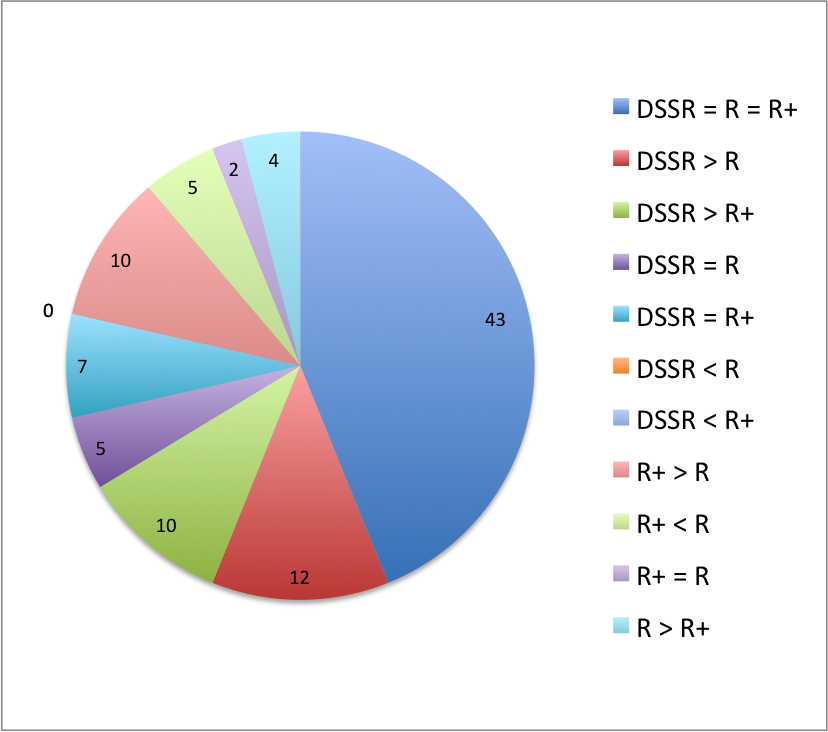
\includegraphics[width=8cm,height=7cm]{pie5.png}
%\caption{Division of result in to categories}
%\label{fig:pie}
%\end{figure}






The first category contain 12 classes where DSSR strategy performs better than R. 
The second category contain 10 classes where DSSR strategy performs better than R+. 
The third category contain 5 classes where DSSR strategy and R performs equally well.
The fourth category contain 7 classes where DSSR and R+ performs equally well. 
The fifth category contain 10 classes where R+ performs better than R.
The sixth category contain 5 classes where R performs better than R+.
The seventh category contain 2 classes where R and R+ performs equally well.
The eighth category contain 4 classes where R performs better than R+.
Category 9 and 10 shows that neither R nor R+ performed better than DSSR strategy.
The last category shows each strategy performing equally well for 43 classes. Expressing in percentage, 72\% classes do not show different behaviours whereas in 28\% of classes, the DSSR strategy performs better than R and R+ strategy. It is interesting to note that in no single case R and R+ strategies performed better than DSSR strategy. This is attributed to the fact that DSSR strategy possess the qualities of R and R+ and has the additional advantage of spot sweeping.

\end{comment}

\subsection{Can we pick the best default strategy between R, R+ and DSSR?}

Analysis of the experimental data reveal that DSSR strategy has an edge over R and R+. This is because of the additional feature of Spot Sweeping in DSSR strategy.

In spite of the better performance of DSSR strategy compared to R and R+ strategies the present study does not provide ample evidence to pick it as the best default strategy because of the overhead induced by this strategy (see next section). Further study might give conclusive evidence. 




%%%%%%%%%%%%%%%%%    DISCUSSION   %%%%%%%%%%%%%%%%%%%%

\section{Discussion}\label{sec:discussion}
In this section we discuss various factors such as the time taken, effect of test duration, number of tests, number of faults in the different strategies and the effect of finding first fault in the DSSR strategy.
\textbf{Time taken to execute an equal number of test cases:}
The DSSR strategy takes slightly more time (up to 5\%) than both pure random and random plus which may be due to maintaining sets of interesting values during the execution. We do not believe that the overhead can be reduced. 

\textbf{Effect of test duration and number of tests on the results:}
All three techniques have the same potential for finding failures. If testing is continued for a long duration then all three strategies will find the same number of unique failures and the results will converge. We suspect however that some of the unique failures will take an extremely long time to be found by using random or random+ only. Further experiments should confirm this point.


\textbf{Effect of number of faults on results:} 
We found that the DSSR strategy performs better when the number of faults is higher in the code. The reason seems to be that when there are more faults, their domains are more connected and DSSR strategy works better. Further studies might use historical data to pick the best strategy.

\textbf{Dependence of DSSR strategy to find the first unique failure early enough:}
During the experiments we noticed that if a unique failure is not found  quickly enough, there is no value added to the list of interesting values and then the test becomes equivalent to random+ testing. This means that better ways of populating failure-inducing values are needed for sufficient leverage to DSSR strategy. As an example, the following piece of code would be unlikely to fail under the current setting:

\begin{lstlisting}
public void test(float value){
 if(value == 34.4445)   10/0;
}
\end{lstlisting}

In this case, we could add constant literals from the SUT to the list of interesting values in a dynamic fashion. These literals can be obtained from the constant pool in the class files of the SUT.

In the example above the value 34.4445 and its surrounding values would  be added to the list of interesting values before the test starts and the DSSR strategy would find the unique failure right away.

\textbf{DSSR strategy and coverage:} Random strategies typically achieve high level of coverage~\cite{Oriol2010}. It might also be interesting to compare R, R+ and DSSR with respect to the achieved coverage or even to use a DSSR variant that adds a new interesting value and its neighbours when a new branch is reached.


\textbf{Threats to validity:} As usual with such empirical studies, the present work might suffer from a non-representative selection of classes.
The selection in the current study is however made through random process and objective criteria, therefore, it seems likely that it would be representative.

The parameters of the study might also have prompted incorrect results. But this is unlikely due to previous results on random testing~\cite{Oriol2012}.



%%%%%%%%%%%%%%%%%    RW   %%%%%%%%%%%%%%%%%%%%

\section{Related Work}\label{sec:rw}

Random testing is a popular technique with simple algorithm but proven to find subtle faults in complex programs and Java libraries~\cite{Pacheco2005, Csallner2004, Claessen2000a}. Its simplicity, ease of implementation and efficiency in generating test cases make it the best choice for test automation~\cite{Hamlet1994}. Some of the well known automated tools based on random strategy includes Jartege~\cite{Oriat2004}, Eclat~\cite{Pacheco2005}, JCrasher~\cite{Csallner2004}, AutoTest \cite{Ciupa2007, Ciupa2008a} and YETI~\cite{Oriol2010, Oriol2012}.

In pursuit of better test results and lower overhead, many variations of random strategy have been proposed~\cite{Chen2010, Chen2005, Chan2002, Chen2004a, Chen2003}. Adaptive random testing (ART), Quasi-random testing (QRT) and Restricted Random testing (RRT) achieved better results by selecting test inputs randomly but evenly spread across the input domain. Mirror ART and ART through dynamic partitioning increased the performance by reducing the overhead of ART. The main reason behind better performance of the strategies is that even spread of test input increases the chance of exploring the fault patterns present in the input domain.

A more recent research study \cite{Yoo2012} stresses on the effectiveness of data regeneration in close vicinity of the existing test data. Their findings showed up to two orders of magnitude more efficient test data generation than the existing techniques. Two major limitations of their study are the requirement of existing test cases to regenerate new test cases, and increased overhead due to ``meta heuristics search'' based on hill climbing algorithm to regenerate new data. In DSSR no pre-existing test cases are required because it utilises the border values from R+ and regenerate the data very cheaply in a dynamic fashion different for each class under test without any prior test data and with comparatively lower overhead. 
  
The random+ (R+) strategy is an extension of the random strategy in which interesting values, beside pure random values, are added to the list of test inputs~\cite{Leitner2007}. These interesting values includes border values which have high tendency of finding faults in the given SUT~\cite{Beizer1990}. Results obtained with R+ strategy show significant improvement over random strategy~\cite{Leitner2007}. DSSR strategy is an extension of R+ strategy which starts testing as R+ until a fault is found then it switches to spot sweeping.

%It is interesting that numerous efforts have been made to discover the fault patterns~\cite{Chen2010, Chen2005, Chan2002, Chen2004a, Chen2003}, etc. but in our knowledge, none has been published on covering/sweeping all the faults lying in a specific pattern once it has been discovered.


A common practice to evaluate performance of an extended strategy is to compare the results obtained by applying the new and existing strategy to identical programs~\cite{Gutjahr1999, Duran1984, Hamlet1990}. Arcuri et al. \cite{Arcuri2012}, stress on the use of random testing as a baseline for comparison with other test strategies. We followed the procedure and evaluated DSSR strategy against R and R+ strategies under identical conditions.

In our experiments we selected projects from the Qualitas Corpus~\cite{Tempero2010} which is a collection of open source java programs maintained for independent empirical research. The projects in Qualitas Corpus are carefully selected that spans across the whole set of java applications~\cite{Oriol2012, Tempero2010a, Tempero2008}.


%%%%%%%%%%%%%%%%%    CONCLUSIONS   %%%%%%%%%%%%%%%%%%%%


\section{Conclusions}\label{sec:conc}
The main goal of the present study was to develop a new random strategy which could find more faults in lower number of test cases. We developed a new strategy named. ``DSSR strategy'' as an extension of R+, based on the assumption that in a significant number of classes, failure domains are contiguous or located closely. The DSS strategy, a strategy which adds neighbouring values of the failure finding value to a list of interesting values, was implemented in the random testing tool YETI to test 60 classes, 30 times each, from Qualitas Corpus with each of the 3 strategies R, R+ and DSSR. The newly developed DSSR strategy uncovers more unique failures than both random and random+ strategies with a 5\% overhead. We found out that for 7 (12\%) classes DSSR was significantly better than both R+ and R, for 8 (13\%) classes DSSR performed similarly to R+ and significantly better than R, while in 2 (3\%) cases DSSR performed similarly to R and significantly better than R+. In all other cases, DSSR, R+ and R do not seem to perform significantly differently. Overall, DSSR yields encouraging results and advocates to develop the technique further for settings in which it is significantly better than both R and R+ strategies.

%%%%%%%%%%%%%%%%%    ACKNOWDLEGEMENT   %%%%%%%%%%%%%%%%%%%%
%\section{Acknowledgments}
% should put it back in final version
%The authors thank the Department of Computer Science, University of York for its financial support with the Departmental Overseas Research Scholarship (DORS) award. We also thanks to Richard Page for his valuable help and generous support.




%
% The following two commands are all you need in the
% initial runs of your .tex file to
% produce the bibliography for the citations in your paper.
\bibliographystyle{abbrv}
\bibliography{sigproc}  % sigproc.bib is the name of the Bibliography in this case
% You must have a proper ".bib" file
%  and remember to run:
% latex bibtex latex latex
% to resolve all references
%
% ACM needs 'a single self-contained file'!
%
%APPENDICES are optional
%\balancecolumns
\end{document}
